%%
% bigish macro to create a foldable table top card
\documentclass{article}
\usepackage{color}
\usepackage[utf8]{inputenc}
\usepackage{graphicx}
\usepackage{rotating}
\usepackage{times}
\usepackage{mdwlist}
\usepackage{epic}
\usepackage[code=Code39,X=.5mm,ratio=2.25,H=1cm]{makebarcode}
\usepackage[a4paper,left=5mm,width=200mm,right=0mm,height=290mm]{geometry}
\setlength{\unitlength}{1mm}
\def\figureBase{../}
\newsavebox\namebox
\newsavebox\rolebox
\newsavebox\tablebox
\newsavebox\voorbeeld
\newsavebox\logobox
\newsavebox\commercialboxnl
\newsavebox\commercialboxen
\newsavebox\barcodebox
\newsavebox\frontbox
\setlength\parsep{0pt}
\setlength\parindent{0pt}
\savebox\voorbeeld{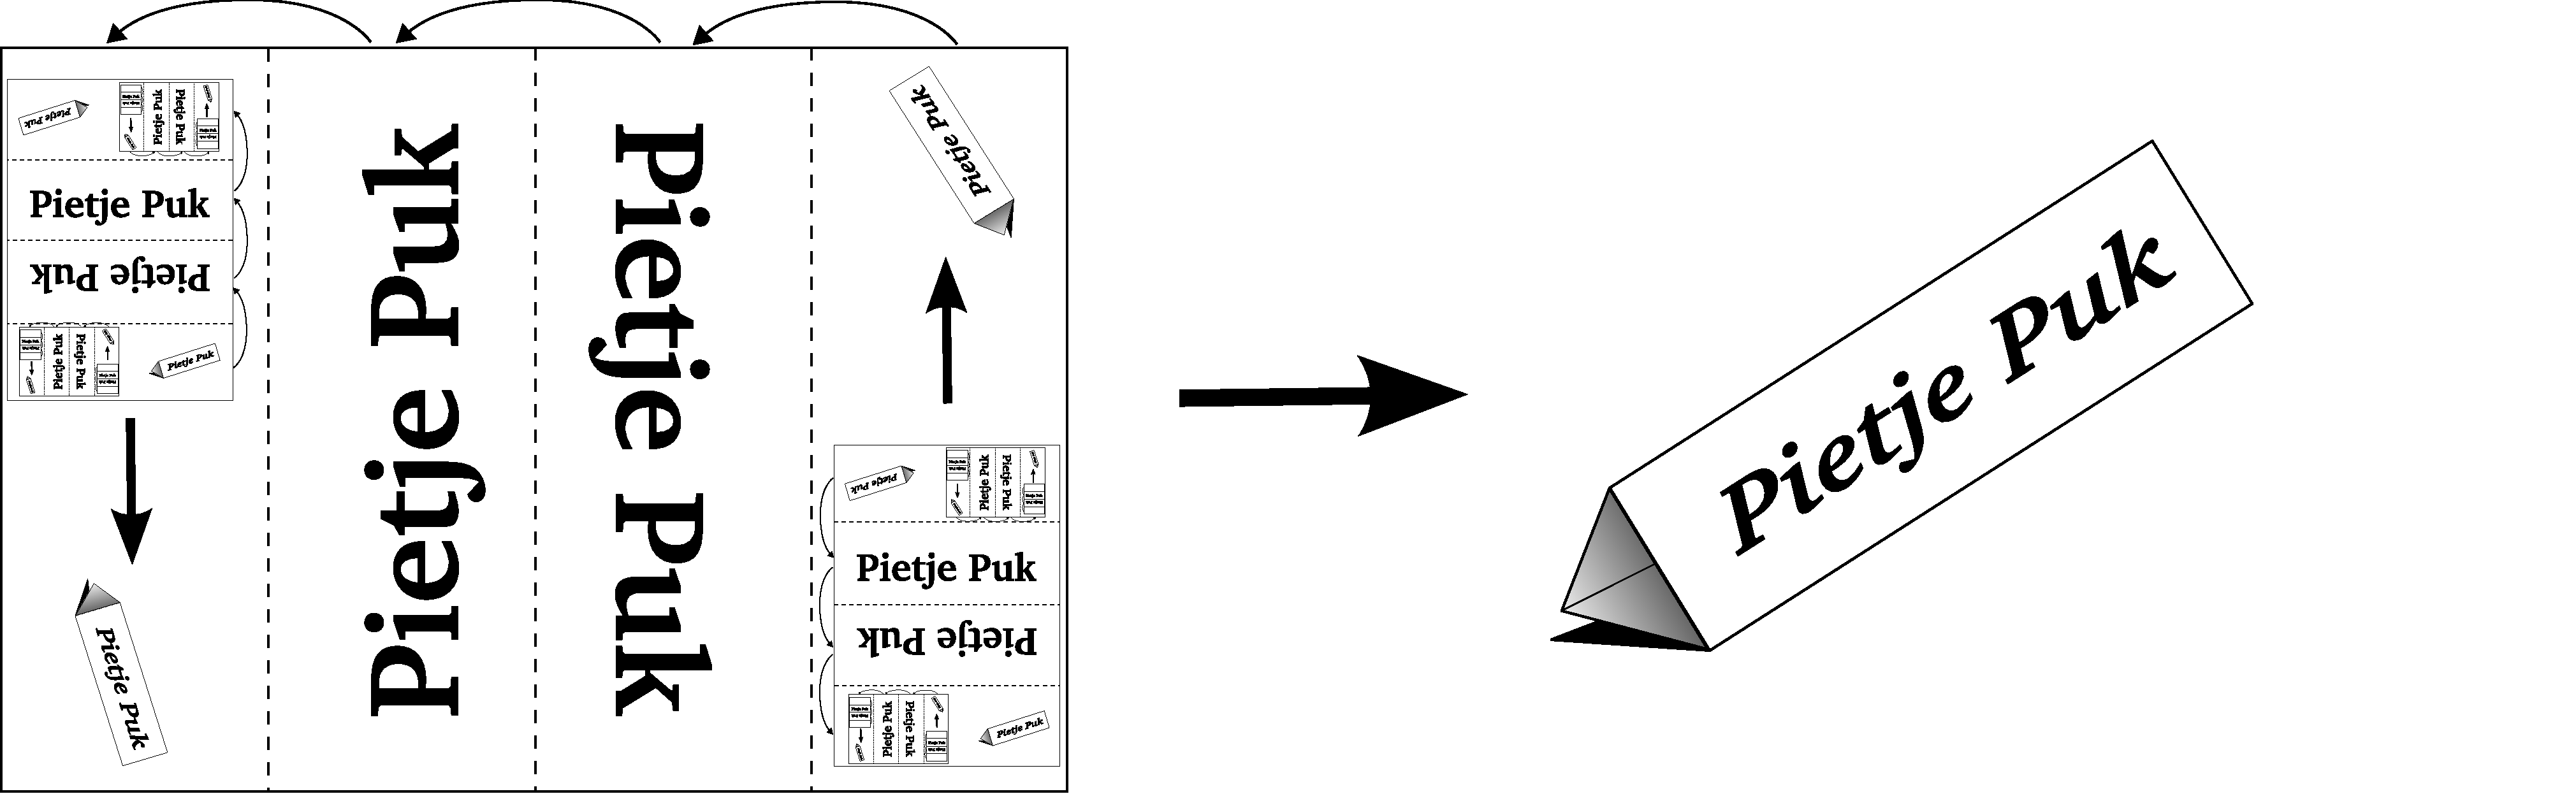
\includegraphics[width=100mm]{\figureBase/figures/Vouwvoorbeeld}}
\savebox\logobox{
\includegraphics[width=30mm]{\figureBase/figures/logo}}
\savebox{\commercialboxnl}[200mm][c]{
\mbox{
\begin{picture}(100,60)
\put(0,60){\large Vouwen volgens voorbeeld:}
\put(0,20){\usebox{\voorbeeld}}
\end{picture}}
\mbox{
\begin{minipage}[b]{70mm}
\raggedright
\sf
\setlength\itemsep{0pt}
Fontys Hogeschool voor Techniek en Logistiek\\
{\em De} plaats voor actie in de techniek.\\
Opleidingen: \\
\begin{itemize*}
\item Mechatronica
\item Software Engineering/Business Informatics
\item Industri\"eel Product Ontwerp
\item Werktuigbouwkunde
\item Logistiek Management
\end{itemize*}
made with \LaTeX
\end{minipage}%
}
}
\savebox{\commercialboxen}[200mm][c]{
\mbox{
\begin{picture}(100,60)
\put(0,50){\large Fould like the example:}
\put(0,6){\usebox{\voorbeeld}}
\end{picture}}
\mbox{
\begin{minipage}[b]{70mm}
\raggedright
\sf
\setlength\itemsep{0pt}
Fontys Hogeschool voor Techniek en Logistiek\\
{\em The} place for action in engineering.\\
Courses in: \\
\begin{itemize*}
\item Mechatronics
\item Software Engineering/Business Informatics
\item Industrial Product Design
\item Mechanical Engineering
\item Logistics Management
\end{itemize*}
made with \LaTeX
\end{minipage}%
}
}
\newcommand\tablecard[4]{
  {% define the content of the boxes
    \savebox{\namebox}[\textwidth][l]{\resizebox{190mm}{!}{{\bf%
        #1%
        }}}% savebox namebox
    \savebox{\rolebox}[\textwidth][l]{\resizebox{!}{12mm}{%
        #2%
        }}% savebox rolebox
    \savebox{\tablebox}[\textwidth][l]{\resizebox{!}{10mm}{%
        #3%
        }}% savebox tablebox
    \savebox{\barcodebox}[.4\textwidth][l]{%
      \begin{minipage}{50mm}
        \barcode{#4}\\#4%
      \end{minipage}
    }% savebox tablebox
%\fbox{%
\savebox{\frontbox}[200mm][c]{
%\fbox{
\begin{picture}(195,68)
\put(0,40){\usebox{\namebox}}
\put(0,20){\usebox{\rolebox}}
\put(0,3){\usebox{\tablebox}}
\put(165,0){\usebox{\logobox}}
\end{picture}
%}
}
%\put(0,0){\large#1}
\begin{picture}(200,290)(0,0)
\put(0,215){\begin{turn}{180}\usebox{\frontbox}\end{turn}}
\put(0,75){\usebox{\frontbox}}
\dottedline{2}(-10,72)(210,72)
\dottedline{2}(-10,145)(210,145)
\dottedline{2}(-10,217)(210,217)
\put(0,5){\usebox{\commercialboxnl}}
\put(15,6){\usebox{\barcodebox}}
\put(0,275){\begin{turn}{180}\usebox{\commercialboxen}\end{turn}}
\put(100,280){\begin{turn}{180}\usebox{\barcodebox}\end{turn}}
\end{picture}
%} % fbox
\clearpage%
  }%
}% tablecard

%%% Local Variables: 
%%% mode: latex
%%% TeX-master: t
%%% End: 
